\documentclass[onecolumn,preprint,superscriptaddress,nofootinbib]{revtex4-1}


\linespread{1.}

%=============================================================================
%\usepackage[margin=1.in]{geometry}
\usepackage{slashed}
\usepackage{graphicx}
\usepackage{amssymb}
\usepackage{mathtools}
\usepackage{bbold}
\usepackage{amssymb,latexsym}
\usepackage{amsmath,amsbsy,bbm}
\usepackage{multirow}
\usepackage[vcentermath]{youngtab}
\usepackage{nicefrac}
\usepackage[perpage]{footmisc}
\usepackage{wrapfig,lipsum,booktabs}
\usepackage{subcaption}
\usepackage{ragged2e}
\DeclareCaptionJustification{justified}{\justifying}
\captionsetup{justification=justified,singlelinecheck=false,labelfont=large}
\usepackage{graphicx}
\usepackage{cjhebrew}

%\usepackage{physics}
\usepackage{floatrow}
\usepackage[dvipsnames]{xcolor} 
%\newfloatcommand{capbtabbox}{table}[][\FBwidth]
%=============================================================================
\newfloatcommand{capbtabbox}{table}[][0.45\textwidth]
%\DefineFNsymbols*{lamportnostar}[math]{\dagger\ddagger\S\P\|{\dagger\dagger}{\ddagger\ddagger}}
%\setfnsymbol{lamportnostar}
%\renewcommand\thefootnote{\fnsymbol{footnote}}
%=============================================================================
\newcommand{\es}{1\text{\scriptsize s}}
\newcommand{\zs}{2\text{\scriptsize s}}
\newcommand*{\mprime}{^{\prime}\mkern-1.2mu}
\newcommand{\largescale}{\ensuremath{\Lambda_\text{Hi}}}
\newcommand{\lc}{\ensuremath{\Lambda_c}}
\newcommand{\fm}{\ensuremath{\,\text{fm}^{-1}}}
\newcommand{\abb}{\mbox{\ensuremath{A\oplus 1}}}
\newcommand{\lec}{C^\Lambda}
\newcommand{\led}{D^\Lambda}
\newcommand{\ddrei}[1]{\delta_{\tiny \Lambda}^{(3)}\!\big(#1\big)}
\newcommand{\wrt}{\textit{wrt.}~}
\newcommand{\etc}{\textit{etc.}~}
\newcommand{\eg}{\textit{e.g.}~}
\newcommand{\ie}{\textit{i.e.}~}
\newcommand{\eftnopi}{\mbox{EFT$(\not \! \pi)$}}
\newcommand{\ve}[1]{\ensuremath{\boldsymbol{#1}}}
\newcommand{\rms}[1]{\ensuremath{\langle r(#1)\rangle}}
\newcommand{\ls}{\ve{L}\cdot\ve{S}}
\newcommand{\be}{\begin{equation}}
\newcommand{\ee}{\end{equation}}
\newcommand{\bra}{\big\langle}
\newcommand{\ket}{\big\rangle}
\newcommand{\hl}{\big\vert}
\newcommand{\vcl}[1]{\ensuremath{\bar{\boldsymbol{r}}_\text{\tiny #1}}}
\newcommand{\vsp}[1]{\ensuremath{\boldsymbol{r}}_\text{\tiny #1}}
\newcommand{\la}{\label}
\newcommand{\Pe}{\text{\cjRL{p|}}}
\newcommand{\figref}[1]{fig.~\ref{#1}}
\newcommand{\tabref}[1]{table~\ref{#1}}
%=============================================================================
\usepackage[normalem]{ulem}


\begin{document}

\title{Multi-fermion systems with contact theories}


\author{M.~Sch{\"a}fer}
\affiliation{Nuclear Physics Institute of the Czech Academy of Sciences, 25069 \v{R}e\v{z}, Czech Republic}
\affiliation{Czech Technical University in Prague, Faculty of Nuclear Sciences and Physical Engineering, B\v{r}ehov\'{a} 7, 11519 Prague 1, Czech Republic}
\author{L.~Contessi} 
\affiliation{Racah Institute of Physics, The Hebrew University, 91904 Jerusalem, 
Israel} 
\affiliation{ESNT, IRFU, CEA, Universite Paris Saclay, F-91191 Gif-sur-Yvette, France} 
\author{J. Kirscher}
\affiliation{Theoretical Physics Division, School of Physics and Astronomy,
The University of Manchester, Manchester, M13 9PL, United Kingdom}
\author{J. Mare\v{s}}
\affiliation{Nuclear Physics Institute of the Czech Academy of Sciences, 25069 \v{R}e\v{z}, Czech Republic\vspace*{2cm}}


%\date{\today}


\begin{abstract}
We demonstrate numerically the universal instability of quantum few-body systems with zero-range
momentum-independent two-body interactions if a mixed-symmetry wave function
is enforced.
Any theory that describes a universality class in which the two-body
scattering length is much larger than any other scale present, exhibits this instability.
We exemplify this with nuclear physics where the feature is realized as the inability
of the leading-order pionless effective field theory to
describe stable states of $A>4$ nuclei.
A finite interaction range is identified as a necessary condition for a stable mixed-symmetry
$A$-body system.
We find that the minimal value of this range depends on the
proximity of a system to unitarity, on the number of its constituents $A$, and on various realizations of discrete scale invariance.
% 
%% state something for the addition of a new scale ?
\end{abstract}

%=============================================================================

\maketitle


\section{Introduction}

Quantum systems with a characteristic two-body scale, like a scattering length $a_0$, much larger than the interaction range $r_0$
develop universal behavior which is independent of the energy scale of the problem and
the details of the interaction.
These universal or scale invariant features can be identified for example in
hadronic molecules, nuclei, and atoms~(see, \eg
Refs.~\cite{Tornqvist:1991ks,Voloshin:2003nt,Braaten:2003he,philli,tjon,PhysRevLett.81.69}) 
where very different degrees of freedom give rise to $r_0/a_0\to 0$\footnote{We adopt the canonical terms: {\it resonant/unitarity} limit
if $|a_0|\to\infty$, and {\it zero-range/contact} limit if $r_0\to0$ with fixed $a_0$.}.
Prominent examples of such universal behavior include the accumulation of infinite bound states at threshold in the three-boson system with a contact two-body interaction~\cite{Efimov:1971zz}~and the associated Thomas collapse~\cite{PhysRev.47.903}.
This collapse represents the emergence of a three-body scale in the absence of any finite two-body scale, and an ensuing breaking of the continuous scale invariance down to a discrete version of it.
Particular realizations of it correspond to specific physical systems, \eg the triton~\cite{Bedaque:1998kg}.
The Tjon~\cite{tjon}~and Phillips~\cite{philli}~correlations, and the spectrum of the multi-boson system~\cite{manybosons} are then consequences of the extended universality beyond three particles and bound states.
All these examples concern states with total spatial symmetry. Very few instances of universal behavior are known for systems which cannot reside in pure $S$-wave states.

Two recent discoveries stand out: 
first, a zero-range theory was shown to stabilize systems of three 
fermions with two components of unequal mass only
if the mass ratio between the two species $\gtrapprox8.2$~\cite{Kartavtsev_2007}.
Second, a zero-range resonant two-body interaction was found to have similar consequences for the stability of a four-body system of particles with equal mass. 
In particular, the universal ratio between the scattering lengths of
two two-component dimers to the fermion-fermion scattering length
implies the unstable nature of the four fermions~\cite{petrov_dimerov, Petrov:2005zz,PhysRevA.92.053624}.
Nucleons, however, are four-component fermions and thus most non-$S$-wave features can only be found for
larger numbers of particles.
Realizing the contact-interaction condition within the effective-field-theory (EFT) framework,
the $^{16}$O nucleus was found unstable with respect to a four-$\alpha$ decay~\cite{Contessi:2017rww}.
Similarly, $^{6}$He was found not to be stabilized by a momentum-independent resonant interaction
while $^{6}$He and $^{16}$O are stable if a $P$-wave attraction is included nonperturbatively~\cite{Gattobigio:2019omi, PhysRevC.98.054301}.
All the above studies hint towards a general characteristic of theories with $r_0/a_0\rightarrow 0$, namely,
the universal prediction of unstable mixed-spatial-symmetry systems ($P$-wave systems, from here on).

In this paper, we analyze precisely this issue: whether universality
excludes stable $P$-wave states in general, and the necessity of an augmentation in order to describe them. 
First, we complement the aforementioned studies of few-nucleon systems with 6-, 7-, and 8-body calculations,
approaching the contact limit with an EFT. 
Subsequently, we attempt to find universal and stable $P$-wave states under the most favorable conditions.
Motivated by Ref.~\cite{Kartavtsev_2007},~in which the binding of two non-interacting identical fermions is induced by a third massive particle, we device a system of $A+1$ particles which includes a pair of identical fermions where $A$ particles form a
massive spatially symmetric core which might give rise to an analogous binding effect. 
As we will show, there is no evidence of $P$-wave binding even in this ideal scenario.
Thus we conclude that the absence of stable $P$-wave states in any system with a unitary
or contact $S$-wave interaction is one of its universal features.

This conjecture affects theoretical descriptions of all systems in this universality class,
arguably most prominently the EFT for nuclei, which, as of now, cannot account for the
observed $P$-wave stability 
and might have to be augmented with an additional constraint.

%=============================================================================
%\vspace{4mm}
\section*{Theory}
The minimal EFT for non-relativistic point particles forming two- and three-body shallow states has been studied extensively (\eg in Refs.\cite{Lepage:1997cs,vanKolck:1999mw, Bedaque:1998kg, Braaten:2004rn, Hammer:2017tjm, Hammer:2019poc}).
The theory is defined as a perturbative series and can be refined systematically to attain a desired accuracy.
Its Hamiltonian formulation at leading order (LO) comprises zero-range two- and three-body vertices which depend on the renormalization parameter~$\Lambda$:
%
\begin{align}
H = - \sum_{i<j} \frac{\hbar^2}{2m}\ve{\nabla}_{ij}^2+ \lec \sum_{i<j}{\delta_\Lambda(\ve{r}_i-\ve{r}_j)} 
\,+\nonumber\\
\led \sum_{ i<j<k \atop \text{cyc} }\delta_\Lambda(\ve{r}_i-\ve{r}_j)\delta_\Lambda(\ve{r}_i-\ve{r}_k).
\label{eq:hamiltonian}
\end{align}
%
In the expansion of any resultant amplitude, the LO is given by all Born
terms depending solely on the coupling constants $\lec$ and $\led$. 
Parameters representing the aforementioned refinements
enter perturbatively at the order given na\"ively by their mass
dimension. 
In this work, a Gaussian regulator 
\mbox{$\delta_\Lambda(\ve{x}) \propto\Lambda^3 e^{-\frac{\Lambda^2}{4}\ve{x}^2}$} is used (such that $\Lambda\propto r_0^{-1}$).
The specific dependence of $\lec$ and $\led$ on $\Lambda$ thus induced, was calibrated to
the energy of a single state in the two- ($B(2)$) and three-body
($B(3)$) system, respectively.
Whether or not the $\Lambda$ convergence of another amplitude depends on the
specific choice for $B(2)$ and $B(3)$ classifies the corresponding observable as
universal or emergent.
The few-body problem is thereby specified at LO with four parameters: the particle's mass
(here, $m=938~$MeV), the number of particles 
(and their statistics),
and the dimer and trimer binding energies.
The possibility of varying the cutoff and/or including sub-leading orders renders the contact EFT
a useful framework 
not only to study the universal regime itself but especially to determine deviations from it.
%%

We use this structure to consider both the nuclear scenario and a class of systems with ($A+1$) equal-mass constituents which contain only one pair of indistinguishable fermions. 
Therefore, a subset of $A$ distinguishable particles can be described by a symmetrical spatial wave function (\eg, the $S$-shell), as stipulated in the introduction.
These arrangements will be referred to as \abb~because this notation highlights the core size $A$.
We approach the unitarity limit in these systems by increasing the ratio \mbox{$\Pe:=B(3)/B(2)$}.
Exact unitarity is realized with $B(2)=0$ ($a_0\rightarrow +\infty$) in combination with $B(3)=1$~MeV, and deviations from it with $B(2)=1$~MeV and $B(3)\in\lbrace3,\,4\rbrace$~MeV.
The nuclear case is renormalized to yield the deuteron and triton binding energies of $B(2)=2.22$~MeV and $B(3)=8.48$~MeV, respectively. 
In accordance with the recent formulation of $S$-shell nuclei in an expansion about the unitarity limit, which is (iso)spin symmetric at LO \cite{Konig:2016utl}, we choose to drop any spin and isospin dependence of the interaction.

The necessary fits for $\led$ employ diagonalizations in bases built with the Stochastic
Variational Method (SVM,~\cite{Suzuki:1631377}) and the
Resonating Group Method (RGM,~\cite{PhysRev.52.1083,hmh-rrgm}). $\lec$ is
determined via a Numerov-type integration of the appropriate one-dimensional
radial Schr\"odinger equation.



%%%%%%%%%%%%%%%%%%%%%%%


%\hspace{2cm}
\newpage
\section*{Results:}


\begin{figure}
\centering
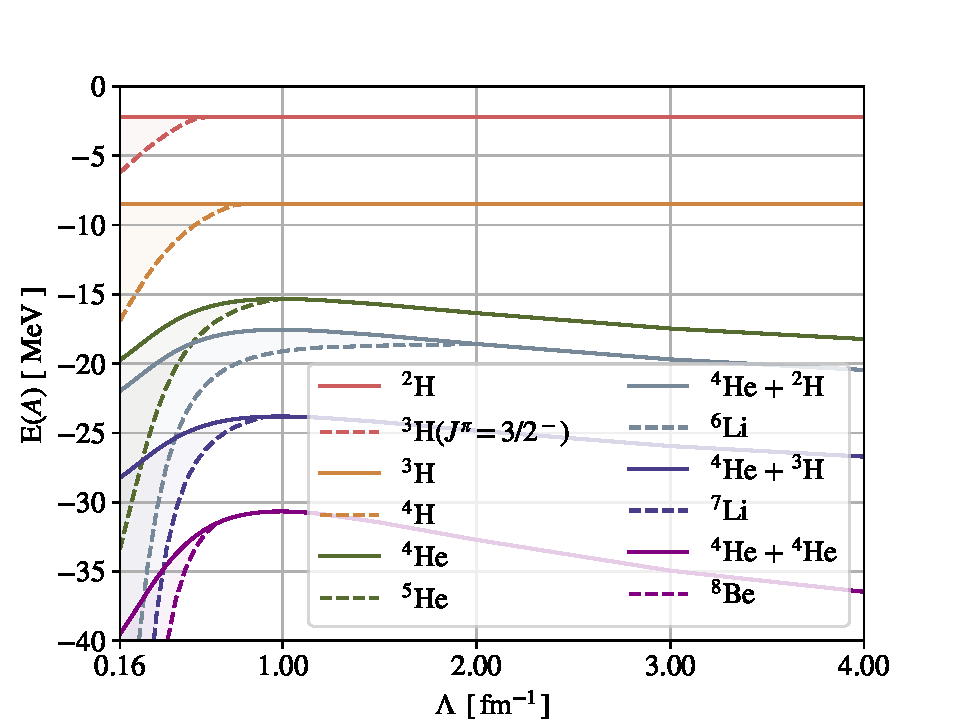
\includegraphics[width=\linewidth]{./Nuclear.pdf} 
\caption{Cutoff dependence of nuclear ground-state energies
obtained in LO~\eftnopi. For $A \leq 4$, solid lines represent nuclei with
spatially symmetric ground-state wave-function components. For $A>4$,
solid lines mark the lowest decay threshold into two spatially symmetric fragments.
The dependence up to $\Lambda\sim 10$~fm$^{-1}$ is in agreement with the expected $E\propto\Lambda^{-1}$ behavior \cite{Bedaque:1998kg, Barnea:2013uqa}.
The large-cutoff region is not shown to improve the readability.}
\label{fig:nuclear}
\end{figure}

Our results, as obtained within the above defined theory
for the lowest energy eigenvalues of nuclear systems of up to eight nucleons, are shown
in \figref{fig:nuclear}.
Particle-stable $P$-wave nuclei (dashed lines) are found only below a critical cutoff $\lc<2\fm$.
For larger cutoffs, \ie shorter-ranged interactions,
the $J^\pi=3/2^-$ state of $^3$H is unstable \wrt a decay into a deuteron plus a neutron, \mbox{$^4\text{H}\to\,^3\text{H} + n$},
\mbox{$^5\text{He}\to\alpha +n$}, \mbox{$^6\text{Li}\to\alpha+{}^2\text{H}$}, \mbox{$^7\text{Li}\to\alpha + {}^3\text{H}$},
 and \mbox{$^8\text{Be}\to \alpha+\alpha$}.
The cutoff value below which a stable state exists is system dependent:

\begin{equation}
\label{eq:lc-order}
\lc(^3\text{H})<\lc(^8\text{Be})<\lc(^4\text{H})<\lc(^7\text{Li})<\lc(^5\text{He})<\lc(^6\text{Li})\;\;.
\end{equation}
%
Na\"ively, we expect three characteristic parameters of a system to control the value of $\lc$:
the total number of particles $A$, the typical size of the smaller of the two decay fragments, and
the number of particles in it.
With the size and the number of particles in the smaller fragment the attraction due to particle
exchange rises, increasing stability even for shorter interaction ranges.
The maximal $\lc$ in relation \eqref{eq:lc-order} is generated by the large
deuteron fragment in ${}^6$Li and demonstrates this effect.
Moreover, with the increase of the total number of particles the quantity of interacting pairs and triplets grows.
Keeping the smaller fragment size constant, we observe
(a discussion follows below \figref{fig:threshold})
that this effect is almost linear for a relatively small number of particles $A \leq 6$.
%
For all considered nuclei, we find $\lc$ to be of the order of the breakdown scale\footnote{We
adopt the canonical estimate of $m_\pi$ for the breakdown scale of \eftnopi~around which
substructure of the nucleons represented by the pion as the lightest meson becomes observable.}
of the \eftnopi.
%
The instability is therefore invariant \wrt renormalization-group (RG)
transformations with $\Lambda\gg m_\pi$.
On the one hand, the LECs of the theory at LO are still sufficient to renormalize these larger
nuclei consistently.
On the other hand, the three-parameter theory postdicts correctly only the experimentally
established instability of nuclei in the
$^3\text{H}(3/2^-),\,^3n,\,^4\text{H},\,^{3,4}\text{Li},\,\text{and}~^5\text{He}$ channels.
The isotopes $^{6,7}\text{Li}$ and $^8$Be with $J^\pi=1^+$, $3/2^-$, and $0^+$, which are known to sustain stable
states\footnote{Without Coulomb repulsion, $^8$Be is considered to be stable ~\cite{AFZAL:1969zz,Higa:2008dn}.}~are
not correctly reproduced in that respect.
%
Interestingly, once a stable $^8$Be ground state is found with $J^\pi=0^+$ at $\Lambda<\lc$ the theory orders excited states in the
rotational spectrum correctly, namely, $0^+$, $2^+$, and $4^+$. 
The latter two states emerge in a form of bound excited states for $\Lambda<0.4~{\rm fm^{-1}}$.

%
\begin{figure}
    \centering
        \centering
        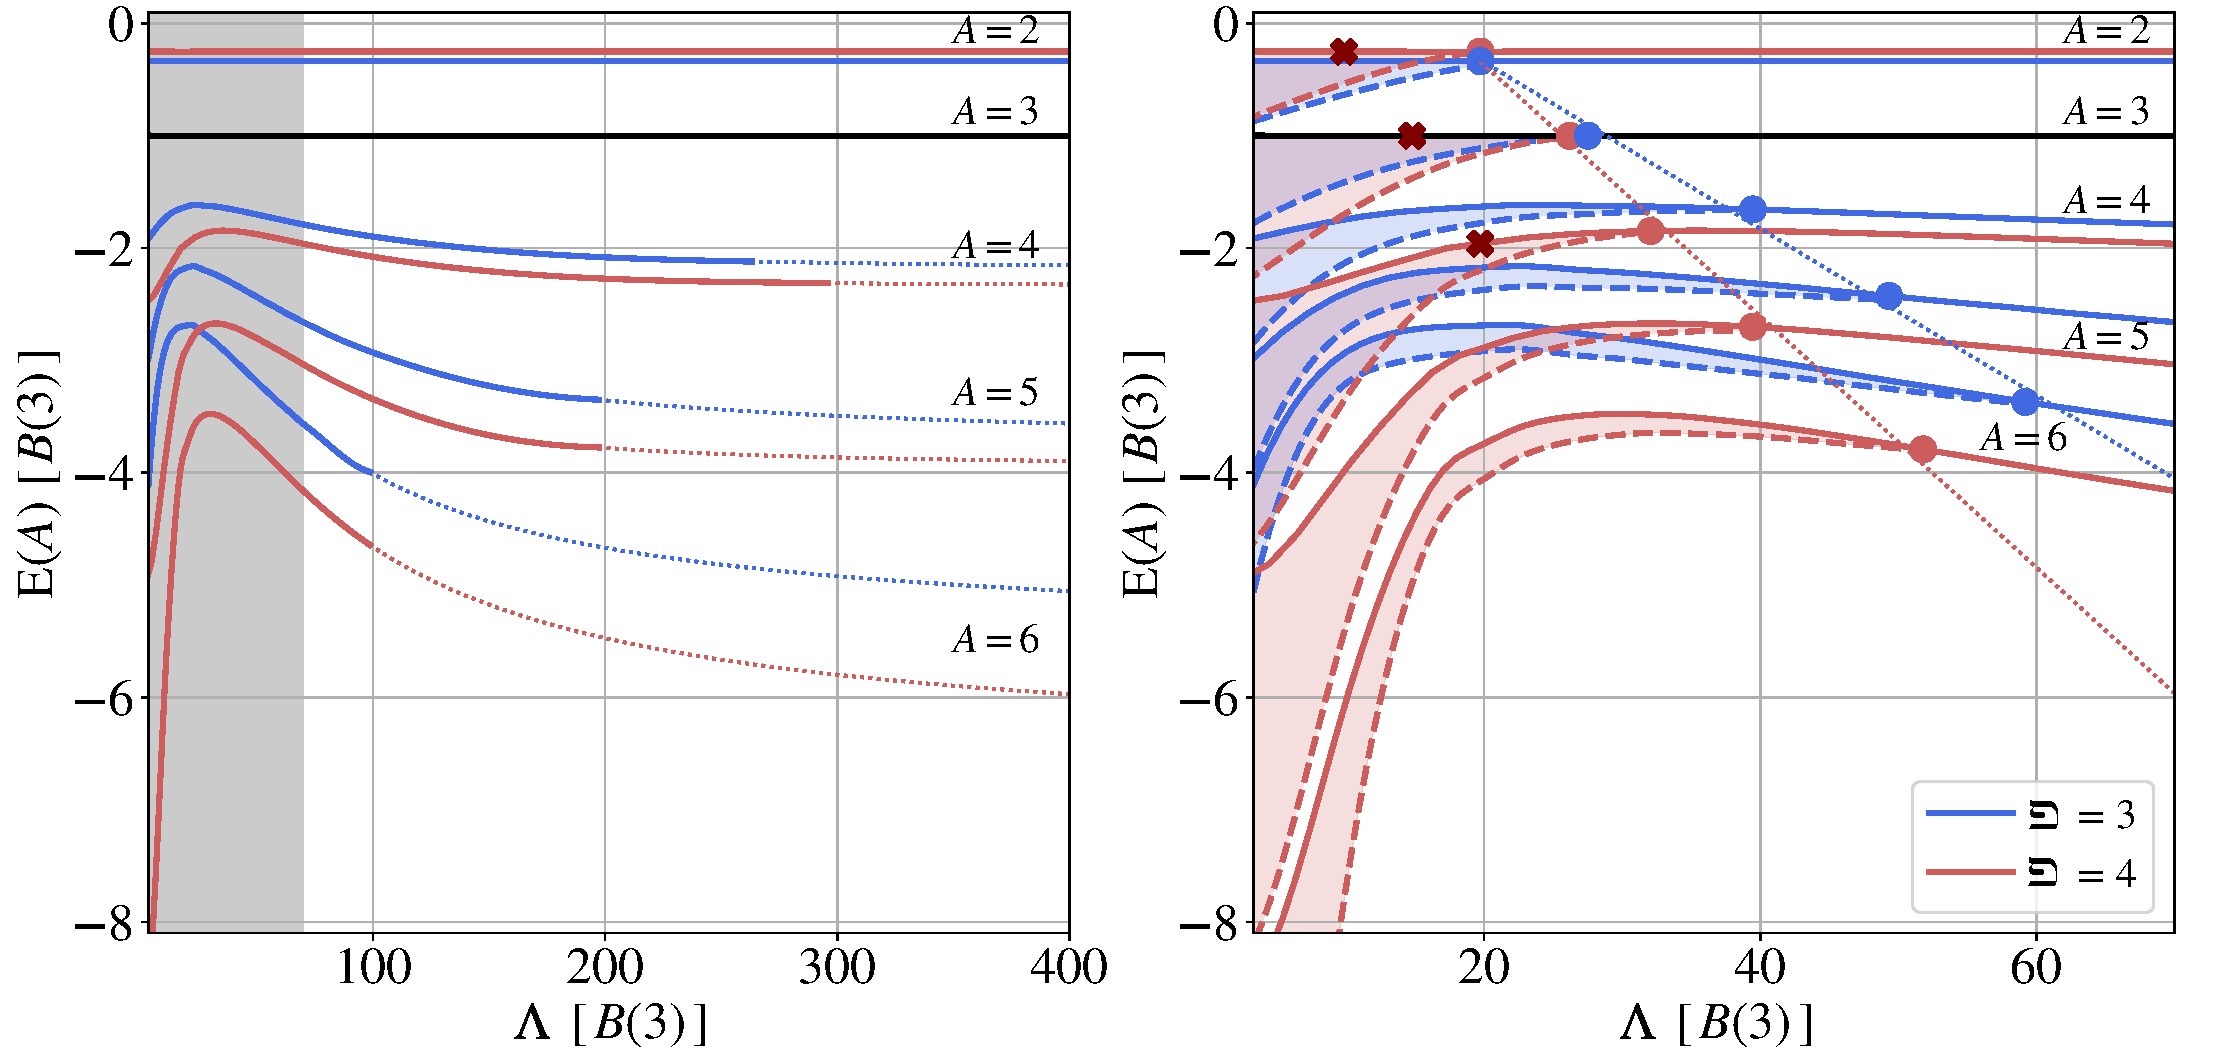
\includegraphics[width=\linewidth]{./new-p-wave} 
        \caption{Left panel: cutoff dependence of ground-state energies of systems comprising $A$ distinguishable fermions with \eqref{eq:hamiltonian}~calibrated to $B(2)=1~$MeV and \mbox{$B(3)\in\lbrace3,4\rbrace~$MeV} (blue and red). Dotted lines denote extrapolation curves. Right panel: small-cutoff region
        (gray area in the left panel) including ground-state energies of \abb~mixed-symmetry systems (dashed lines). The linear-in-$A$ trend of critical cutoffs $\lc$ (dots) is marked
        by dotted lines. Red crosses indicate critical cutoffs if the scattering volume is zero.}
        \label{fig:threshold}
\end{figure} 
%

%
We now generalize the above nuclear $P$-wave instability of the $\eftnopi$~
and renormalize to values of $\Pe$ which parametrize systems arbitrarily close to unitarity.
Removing the finite two-body scale by recalibrating EFTs at unitarity ($\Pe\rightarrow \infty$),
we obtain
the ratio $B(4)/B(3)$ in agreement with Refs.~\cite{Hammer:2006ct,2009NatPh...5..417V}~as a
benchmark.
In addition, \mbox{$B(A)/B(3)\Big\vert_{\Pe=3}<B(A)/B(3)\Big\vert_{\Pe=4}$}, indicating that the
universal ratios between the $A$- and 3-body energies are approached from below when taking the
unitary limit.

In the left panel of \figref{fig:threshold},
our results for the cutoff dependence of binding energies of spatially symmetric systems is shown.
For large cutoffs, a $\Lambda^{-1}$ function
represents a visibly appropriate extrapolation of the results (dotted curves)
which was consistently found in Ref.~\cite{Betzalel:2016} for $A=4$-, 5-, and 6-boson systems.
Beyond distinguishable particles, we find systems with \abb~symmetry not stable in states with
total orbital angular momentum $L_\text{total}=0$.
This confirms the intuitive demand for mixed spatial symmetry due to the presence
of an identical fermionic pair.
When projecting the spatial component of the wave function onto \mbox{$L_\text{total}=1$},
we find the \abb~systems for $A$ between 2 and 6 to sustain stable states \mbox{($B(\abb)>B(A)$)}
for small cutoffs
(right panel of \figref{fig:threshold}~highlighting the gray-shaded
cutoff interval in the left panel). 
Approaching the contact limit by increasing the cutoff, the \abb~systems become
unbound at some critical value $\lc$ (filled dots).
For fixed $\Pe$, $\lc$'s increase approximately linearly with the system size:
\mbox{$\lc\propto A \leq 6$} (dotted lines).

\begin{figure}
\centering
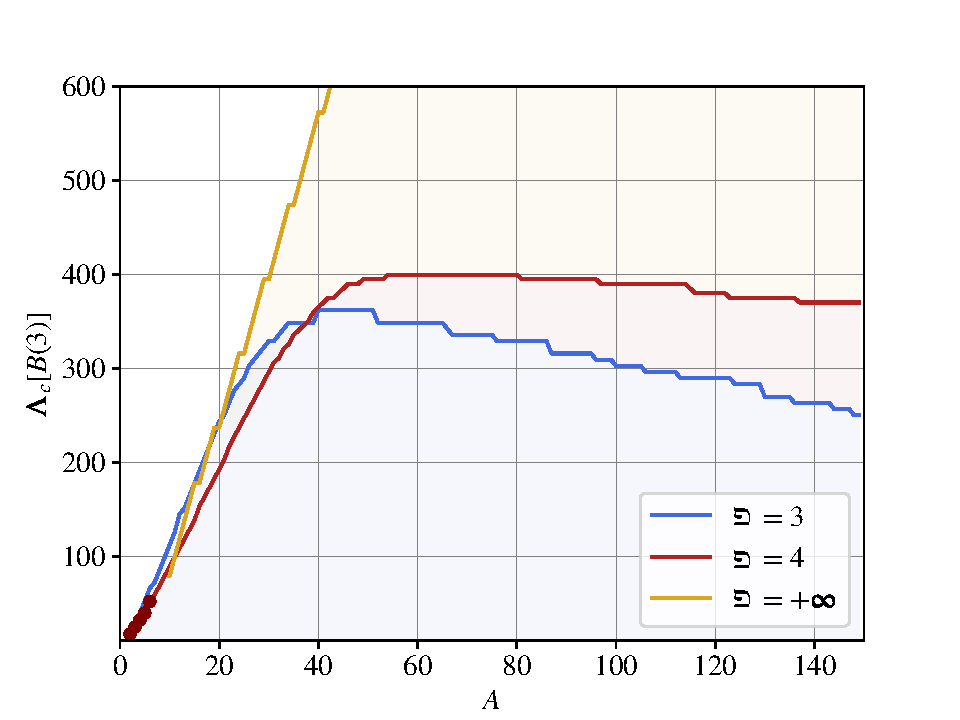
\includegraphics[width=\linewidth]{./RGM-pe-v1.pdf} 
\caption{Dependence of the critical cutoff $\lc$ on the number of core particles
$A$. SVM few-body results (red dots) are shown for $A\leq6$ and $B(3)=4~$MeV (see right panel of \figref{fig:threshold})~along with single-channel resonating-group approximations for $A<150$ (lines). The unitarity limit
(yellow) was realized with $B(2)=0$ ($a_0\rightarrow+\infty$) and $B(3)=1~$MeV and deviations from it
with $B(2)=1~$MeV and $B(3)\in\lbrace3,4\rbrace~$MeV (blue, red). 
In the shaded regions, the respective theories do sustain stable \abb~states,
while systems above the lines are unstable.
The step-like change in the curves results from a numerical criterion for the onset of binding and
can be removed systematically. }
\label{fig:RGM}
\end{figure}

Results presented thus far, substantiate the hypothesis of unstable $P$-wave states for $A\leq 6$, only. 
To investigate conceivable deviations from
the linear dependence of $\lc$ on $A$, particularly in form of divergences, we employ a two-fragment
local single-channel resonating-group approximation
(to be detailed in upcoming communication as an extension of Refs.~\cite{PhysRev.52.1083,Naidon_2016}). 
This expansion formulates the (\abb)-body system as a two-body problem of a ``frozen'' core with $A$ particles and the
fermion which is expelled out of the $S$-wave Pauli shell.
The halo character of the systems under consideration motivates a one-parameter representation of the symmetric core as a product of harmonic oscillator ground states, because the increasingly large gap between $B(A)$ and $B(A-1)$ does not allow for a core excitation
by the out-of-shell particle.
For $A \leq 7$, this parameter is fitted to the SVM results for the rms radius of the core.
For larger $A$, we match the core wave function with the liquid drop model formula $r_\text{rms}\propto A^{1/3}$ as 
it was found to be a good description for such systems in Ref.~\cite{manybosons}.

Away from unitarity, we find $\lc(A)$ to abandon the linear increase found for small $A$.
$\lc$ increases up to a maximum number of particles $A^*$, while this maximum and the associated $\lc(A^*)$
both increase with $\Pe$ (compare maxima of the blue and red curves in \figref{fig:RGM}). At unitarity,
we find a linear dependence up to $A>100$.
The existence of $A^*$ and the deviation from the linear $\Lambda_c\propto A$ relation thus appears to be an effect of deviating from unitarity.
In combination with the microscopic results, this confirms the main hypothesis of this work, namely,
that a system at unitarity cannot
support stable states in the zero-range limit if it contains indistinguishable fermions.

Revisiting nuclear physics as a specific incarnation of this general class of systems,
its description within the LO \eftnopi~will not contain stable states heavier than $^4$He.
Consequently, such nuclei, and all other $P$-wave systems with physical stable states
belong to a different universality class which is defined by at least one new scale.
A first step to identify such scale is to analyse the mechanism behind the stability of the $P$-wave systems for $\Lambda<\lc$.
Of all artefacts introduced by the finite range of the regulated contact interaction,
a finite effective range in the two-body $S$-wave channel and a non-zero attractive two-body $P$-wave interaction are expected to dominate. 
Both contribute to the attraction in the \abb~system but their relative significance is obscure.
In other words, the finite-range interaction does not only describe a large $S$-wave scattering length but
also other finite parameters of the effective-range expansion as the effective range $r_0$ and the scattering volume $a_1$.
To shed light on their relative importance, we project the two-body interaction into even partial waves in order to eliminate the effect of the scattering volume.
The resultant reduction of $\lc$ for all $A$ is significant compared with its
magnitude (red crosses in \figref{fig:threshold}) which is now solely an effect of
even-partial-wave finite-range artefacts. 
Besides this decrease in $\lc$, the $P$-wave binding energy is also reduced by a substantial amount
as a consequence of the removal of the odd-partial-wave interactions.
We infer from these results a similar significance of the finite $r_0$ and $a_1$ for the stability of the nuclear $P$-wave systems, and therefore we cannot identify the new scale
with either of them conclusively.
%

%%%%%%%
%%%%%%%
In addition to the above, we analyze another crucial aspect in the course of the
formulation of the \eftnopi~for large systems.
In principle, the \eftnopi~at LO must yield only the analytic structure of any scattering amplitude
in its range of validity. Convergence of quantitative corrections will be accounted for at
higher orders.
However, whether or not a tighter constraint must hold, namely, that the LO theory should
already describe the correct character of a state (bound, virtual, or resonant) is an open question.
To resolve this, the possibility of transforming a scattering state into a stable
one (or vice-versa) by the insertion of a \textit{perturbative} sub-leading contribution must be addressed.
Without a way to change the pole character perturbatively or if the shallow state even does not exist at all,
only a non-perturbative insertion can provide the stability demanding, however, 
an alteration of the power-counting.
It is, therefore, essential to assess if $P$-states remain shallow and renormalized
after their change of character from stable to unstable as induced by a decreasing interaction range.
As a first step, we confirm the expectation that at unitarity a shallow $2\oplus1$ pole is not fixed to a finite energy.
As for a scale-invariant system the resonance pole must not represent a scale and thus its location should either
merge with the threshold branch cut or diverge for $\Lambda\to\infty$\footnote{We thank U.~van~Kolck for clarifying discussions on this issue.}.
In the first case, three-body $P$-wave unitarity would be a universal consequence of the resonant two-body interaction. 
In the second case, the pole is an unphysical artefact which disappears with the regulator.
Our numerical results exhibit the latter behavior. Specifically, the $2\oplus1$ bound-state pole for $\Lambda<\lc$ hits threshold at $\lc$ and
moves away from it for $\Lambda>\lc$.
However, for $A>2$, scale invariance is broken, and the associated emergence of a scale could in principle
pin the resonance to a finite energy. The pole trajectory for $A>2$ could thus be qualitatively different and
it remains to be calculated in order to advance the development of a contact EFT for $P$-wave systems.



\section*{Conclusion}

We employ a three-parameter non-relativistic contact EFT at LO to describe $P$-wave nuclei with up to eight nucleons.
We find no stable states for these nuclei if the cutoff-renormalization scale of the theory exceeds a system-dependent critical value.
In addition to nucleons with their large but finite scattering length, we find systems which are arbitrarily close to unitarity and realize
discrete scale invariance in multiple ways equally unstable for large enough cutoffs, \ie in the zero-range limit.
We conclude that systems whose dynamics is given by momentum-independent two- and three-body contact terms
constrained by spatially totally symmetric dimer and trimer states, are stable only if their spatial state is totally symmetric.
States of mixed symmetry, as enforced by the presence of identical fermions in a system, are in turn predicted to be universally unstable. 

In order to generalize this result and to assess the role of the ratio of the number of distinguishable particles versus identical
fermions in the system, we analyse ($A+1$)-body equal-mass systems with only one pair of identical fermions within the EFT framework.
Thereby, we enforce a momentum-less contact interaction between all the particle pairs and triplets.
Although, the weakening of the potential attraction due to a single out-of-$S$-shell particle is minimal,
the disintegration into a totally symmetric $A$-body core of distinguishable particles
and a free one is observed if the interaction cutoff is increased beyond a critical value.
We assess the dependence of this critical cutoff on the system size $A+1$ and the proximity to unitarity.
For any non-unitary interaction, the critical range increases with $A$ up to a maximum before decreasing from thereon, while in the unitary
case it rises linearly up to at least $A\sim100$.
In the latter case, this dependence suggests that for any finite-range interaction a number of particles can be found which realizes a stable $P$-wave composite.
Moreover, as the dependence on $A$ does not indicate a convergence of the critical range to zero
for any of the analysed systems, the absence of stable mixed-symmetry states in the contact limit
is one logical conclusion.
Therefore, for a future refined version of an EFT which can be applied to systems with stable states of mixed symmetry,
nuclei in particular, we assess the effect of additional constraints on the theory:
a finite two-body $S$-wave effective-range, or a finite two-body $P$-wave scattering volume. 
Both were found of similar importance for the binding, and our study is thus inconclusive and cannot give preference to one over the other.
Moreover, the way these corrections should be treated -- as a perturbation or in
a non-perturbative fashion -- remains an open question.
Finally, we touch upon the problem that only shallow RG-stable resonance poles in the
spectrum of the EFT at LO may potentially be converted into stable states with perturbative
insertions of sub-leading operators.
If such poles contrarily leave the convergence radius of the theory in the course of the RG evolution, which is what we find for the $2\oplus1$ system, they must be created non-perturbatively.
The answer will eventually allow for a universal understanding of seemingly very different fields,
in which as of now, only Bose-like properties can be paralleled.

\vspace{5mm}
\paragraph*{Acknowledgments}
We thank N.~Barnea,  M.~Birse, U.~van Kolck, N.~Walet for insightful
discussions.
M.S. and J.M. were supported by the Czech Science Foundation GACR Grant No.19-19640S.
L.C. and J.K. acknowledge support from ``Espace de Structure et de r\'eactions
Nucl\'eaire Th\'eorique'' (ESNT, http://esnt.cea.fr) at CEA-Saclay, where this work
was partially carried out.
L.C. was also supported by the Pazy Foundation and by the
Israel Science Foundation Grant No. 1308/16.

%=============================================================================

\newpage

\bibliographystyle{ieeetr}
\bibliography{Thebibliography.bib}
\end{document}
\end{document}
